%%
%% This is file `sample-sigplan.tex',
%% generated with the docstrip utility.
%%
%% The original source files were:
%%
%% samples.dtx  (with options: `all,proceedings,bibtex,sigplan')
%% 
%% IMPORTANT NOTICE:
%% 
%% For the copyright see the source file.
%% 
%% Any modified versions of this file must be renamed
%% with new filenames distinct from sample-sigplan.tex.
%% 
%% For distribution of the original source see the terms
%% for copying and modification in the file samples.dtx.
%% 
%% This generated file may be distributed as long as the
%% original source files, as listed above, are part of the
%% same distribution. (The sources need not necessarily be
%% in the same archive or directory.)
%%
%%
%% Commands for TeXCount
%TC:macro \cite [option:text,text]
%TC:macro \citep [option:text,text]
%TC:macro \citet [option:text,text]
%TC:envir table 0 1
%TC:envir table* 0 1
%TC:envir tabular [ignore] word
%TC:envir displaymath 0 word
%TC:envir math 0 word
%TC:envir comment 0 0
%%
%%
%% The first command in your LaTeX source must be the \documentclass
%% command.
%%
%% For submission and review of your manuscript please change the
%% command to \documentclass[manuscript, screen, review]{acmart}.
%%
%% When submitting camera ready or to TAPS, please change the command
%% to \documentclass[sigconf]{acmart} or whichever template is required
%% for your publication.
%%
%%
\documentclass[sigplan,screen]{acmart}

%%
%% \BibTeX command to typeset BibTeX logo in the docs
\AtBeginDocument{%
  \providecommand\BibTeX{{%
    Bib\TeX}}}

%% Rights management information.  This information is sent to you
%% when you complete the rights form.  These commands have SAMPLE
%% values in them; it is your responsibility as an author to replace
%% the commands and values with those provided to you when you
%% complete the rights form.
\setcopyright{acmlicensed}
\copyrightyear{2024}
\acmYear{2018}
\acmDOI{XXXXXXX.XXXXXXX}

%% These commands are for a PROCEEDINGS abstract or paper.
\acmConference[Cloud computing e infraestructura para Big Data]{Make sure to enter the correct
  conference title from your rights confirmation emai}{Agosto 31-08,
  2024}{Santa Cruz, Bolivia}
%%
%%  Uncomment \acmBooktitle if the title of the proceedings is different
%%  from ``Proceedings of ...''!
%%
%%\acmBooktitle{Woodstock '18: ACM Symposium on Neural Gaze Detection,
%%  June 03--05, 2018, Woodstock, NY}
\acmISBN{978-1-4503-XXXX-X/18/06}


%%
%% Submission ID.
%% Use this when submitting an article to a sponsored event. You'll
%% receive a unique submission ID from the organizers
%% of the event, and this ID should be used as the parameter to this command.
%%\acmSubmissionID{123-A56-BU3}

%%
%% For managing citations, it is recommended to use bibliography
%% files in BibTeX format.
%%
%% You can then either use BibTeX with the ACM-Reference-Format style,
%% or BibLaTeX with the acmnumeric or acmauthoryear sytles, that include
%% support for advanced citation of software artefact from the
%% biblatex-software package, also separately available on CTAN.
%%
%% Look at the sample-*-biblatex.tex files for templates showcasing
%% the biblatex styles.
%%

%%
%% The majority of ACM publications use numbered citations and
%% references.  The command \citestyle{authoryear} switches to the
%% "author year" style.
%%
%% If you are preparing content for an event
%% sponsored by ACM SIGGRAPH, you must use the "author year" style of
%% citations and references.
%% Uncommenting
%% the next command will enable that style.
%%\citestyle{acmauthoryear}
\usepackage{tabularx}
\usepackage{graphicx}
\usepackage[spanish]{babel}

\newcommand{\staricon}[1]{
    \begin{tikzpicture}[scale=#1]
        \filldraw[fill=yellow, draw=black] 
        (0,0) -- (0.2,0.6) -- (0.6,0.6) -- (0.3,0.9) -- (0.4,1.4) -- (0,1.1) -- (-0.4,1.4) -- (-0.3,0.9) -- (-0.6,0.6) -- (-0.2,0.6) -- cycle;
    \end{tikzpicture}
}

%%
%% end of the preamble, start of the body of the document source.
\begin{document}

%%
%% The "title" command has an optional parameter,
%% allowing the author to define a "short title" to be used in page headers.
\title{Visualizers: Athena vs. Looker Studio}

%%
%% The "author" command and its associated commands are used to define
%% the authors and their affiliations.
%% Of note is the shared affiliation of the first two authors, and the
%% "authornote" and "authornotemark" commands
%% used to denote shared contribution to the research.
\author{Bravo Peña}
\author{Darlyn}
\affiliation{
  \institution{UAGRM}
  \city{Santa Cruz}
  \country{Bolivia}
}
\email{contact@bpdarlyn.com}

\author{Torrejón Mendez}
\author{Joel Gabriel}
\affiliation{
  \institution{UAGRM}
  \city{Santa Cruz}
  \country{Bolivia}
}
\email{joel.torrejon.mendez@gmail.com}

\author{Valle Tamayo}
\author{Brandon Jason}
\affiliation{
  \institution{UAGRM}
  \city{Santa Cruz}
  \country{Bolivia}}
\email{bjvtamayo78@gmail.com}
%%
%% By default, the full list of authors will be used in the page
%% headers. Often, this list is too long, and will overlap
%% other information printed in the page headers. This command allows
%% the author to define a more concise list
%% of authors' names for this purpose.
\renewcommand{\shortauthors}{Bravo - Torrejón - Valle}

%%
%% The code below is generated by the tool at http://dl.acm.org/ccs.cfm.
%% Please copy and paste the code instead of the example below.
%%
% \begin{CCSXML}
% <ccs2012>
%  <concept>
%   <concept_id>00000000.0000000.0000000</concept_id>
%   <concept_desc>Do Not Use This Code, Generate the Correct Terms for Your Paper</concept_desc>
%   <concept_significance>500</concept_significance>
%  </concept>
%  <concept>
%   <concept_id>00000000.00000000.00000000</concept_id>
%   <concept_desc>Do Not Use This Code, Generate the Correct Terms for Your Paper</concept_desc>
%   <concept_significance>300</concept_significance>
%  </concept>
%  <concept>
%   <concept_id>00000000.00000000.00000000</concept_id>
%   <concept_desc>Do Not Use This Code, Generate the Correct Terms for Your Paper</concept_desc>
%   <concept_significance>100</concept_significance>
%  </concept>
%  <concept>
%   <concept_id>00000000.00000000.00000000</concept_id>
%   <concept_desc>Do Not Use This Code, Generate the Correct Terms for Your Paper</concept_desc>
%   <concept_significance>100</concept_significance>
%  </concept>
% </ccs2012>
% \end{CCSXML}

% \ccsdesc[500]{Do Not Use This Code~Generate the Correct Terms for Your Paper}
% \ccsdesc[300]{Do Not Use This Code~Generate the Correct Terms for Your Paper}
% \ccsdesc{Do Not Use This Code~Generate the Correct Terms for Your Paper}
% \ccsdesc[100]{Do Not Use This Code~Generate the Correct Terms for Your Paper}

%%
%% Keywords. The author(s) should pick words that accurately describe
%% the work being presented. Separate the keywords with commas.
% \keywords{Do, Not, Us, This, Code, Put, the, Correct, Terms, for,
%   Your, Paper}
%% A "teaser" image appears between the author and affiliation
%% information and the body of the document, and typically spans the
%% page.
\begin{teaserfigure}
  
\includegraphics[width=\textwidth]{images/logo_soe.png}
  \Description{Enjoying the baseball game from the third-base
  seats. Ichiro Suzuki preparing to bat.}
  \label{fig:teaser}
\end{teaserfigure}

\received{20 February 2007}
\received[revised]{12 March 2009}
\received[accepted]{5 June 2009}

%%
%% This command processes the author and affiliation and title
%% information and builds the first part of the formatted document.
\maketitle

% Document content
\section{Introducción}
ACM's consolidated article template, introduced in 2017, provides a
consistent \LaTeX\ style for use across ACM publications, and
incorporates accessibility and metadata-extraction functionality
necessary for future Digital Library endeavors. Numerous ACM and
SIG-specific \LaTeX\ templates have been examined, and their unique
features\cite{ibm-sl} incorporated into this single new template.

If you are new to publishing with ACM, this document is a valuable
guide to the process of preparing your work for publication. If you
have published with ACM before, this document provides insight and
instruction into more \cite{ibm-ml} recent changes to the article template.

The ``\verb|acmart|'' document class can be used to prepare articles
for any ACM publication --- conference or journal, and for any stage
of publication, from\cite{ibm-usl} review to final ``camera-ready'' copy, to the
author's own version, with {\itshape very} few changes to the source.

\section{Data Visualization}
La visualización de datos es la representación de datos mediante el
uso de gráficos comunes, como diagramas, gráficos, infografías e 
incluso animaciones. Estas presentaciones visuales de información
comunican relaciones complejas entre datos y perspectivas basadas
en datos de una manera fácil de entender. \cite{ibm-data-visualization}


\subsection{Importancia}
Las empresas modernas suelen procesar grandes volúmenes de datos
procedentes de diversas fuentes, como las siguientes:

\begin{itemize}
  \item {\textbf{Sitios web internos y externos}}
  \item {\textbf{Dispositivos inteligentes}}
  \item {\textbf{Redes sociales}}
  \item {\textbf{Sistemas internos de recopilación de datos}}
\end{itemize}

Sin embargo, los datos sin procesar pueden ser difíciles de
comprender y utilizar. Por ello, los científicos de datos preparan
y presentan los datos en el contexto adecuado. Les dan una forma
visual para que los responsables de la toma de decisiones puedan
identificar las relaciones entre los datos y detectar patrones o
tendencias ocultas. La visualización de datos crea historias que
hacen avanzar la inteligencia empresarial y respaldan la toma de
decisiones basada en datos y la planificación estratégica.

\subsection{Beneficios}
Algunos beneficios de la visualización de datos son los siguientes:

\begin{itemize}
  \item {\textbf{Toma de decisiones estratégicas :}} Las partes interesadas
  clave y la alta dirección utilizan la visualización de datos para interpretarlos
  de forma significativa. Ahorran tiempo gracias a un análisis de datos más
  rápido y a la capacidad de visualizar el panorama general. Por ejemplo,
  pueden identificar patrones, descubrir tendencias y obtener información
  para mantenerse por delante de la competencia.
  \item {\textbf{Servicio al cliente mejorado :}} La visualización de datos
  resalta las necesidades y deseos de los clientes mediante una representación
  gráfica. Puede identificar deficiencias en su servicio al cliente, mejorar
  estratégicamente los productos o servicios y reducir las ineficiencias operativas.
  \item {\textbf{Mayor compromiso de los empleados :}} Las técnicas de visualización
  de datos son útiles para comunicar los resultados del análisis de datos a un
  equipo grande. Todo el grupo puede visualizar los datos en conjunto para
  desarrollar objetivos y planes comunes. Pueden utilizar el análisis visual para medir
  los objetivos y el progreso y mejorar la motivación del equipo. Por ejemplo, un
  equipo de ventas trabaja en conjunto para aumentar la altura de su gráfico de barras
  de ventas en un trimestre.
\end{itemize}

\subsection{Mejores prácticas}
Con tantas herramientas de visualización de datos disponibles, también ha aumentado
la visualización de información ineficaz. La comunicación visual debe ser simple
y deliberada para garantizar que la visualización de datos ayude a su público
objetivo a llegar a la información o conclusión deseada. Las siguientes prácticas
recomendadas pueden ayudar a garantizar que la visualización de datos sea útil
y clara:

\begin{itemize}
  \item {\textbf{Conozca a su audiencia :}} Piense para quién está diseñada su
  visualización y luego asegúrese de que la visualización de datos se ajuste a
  sus necesidades.
  \item {\textbf{Elija un elemento visual eficaz :}} Existen elementos visuales
  específicos diseñados para tipos específicos de conjuntos de datos. Por ejemplo,
  los diagramas de dispersión muestran bien la relación entre dos variables,
  mientras que los gráficos de líneas muestran bien los datos de series temporales.
  Asegúrese de que el elemento visual realmente ayude a la audiencia a comprender
  la idea principal.
  \item {\textbf{Manténgalo simple :}} Las herramientas de visualización de datos
  pueden facilitar la incorporación de todo tipo de información a su elemento visual.
  Sin embargo, el hecho de que pueda hacerlo no significa que deba hacerlo. En la
  visualización de datos, debe ser muy deliberado con respecto a la información
  adicional que agrega para centrar la atención del usuario.
\end{itemize}
\section{MicrosoftPower BI}
Microsoft Power BI es una plataforma de visualización de datos utilizada principalmente con fines 
de inteligencia empresarial. Power BI son las siglas de Power Business Intelligence y se refiere a 
un conjunto de herramientas de software y conectores que le ayudan a transformar datos de múltiples 
fuentes en información procesable.

Diseñado para ser utilizado por profesionales de negocios con diferentes niveles de conocimiento de 
datos, el tablero de Power BI es capaz de informar y visualizar datos en una amplia gama de estilos 
diferentes, incluyendo gráficos, mapas, tablas, diagramas de dispersión, y mucho más. \cite{power-bi-visualization} 


\subsection{Carácteristicas}

\subsubsection{Usabilidad}
La interfaz amigable de Power BI y su fácil navegación permiten que los usuarios de negocios no técnicos 
tengan una curva de aprendizaje simple, lo que les permite crear visualizaciones de datos con unos pocos clics y sin experiencia en programación.

\subsubsection{Asequibilidad.} 
Power BI se ofrece a través de diferentes planes de precios para que las empresas de todos los tamaños 
puedan aprovechar sus capacidades sin preocuparse demasiado por las limitaciones presupuestarias.

\subsubsection{Visualizaciones.} 
Los líderes empresariales utilizan la narración de datos y las visualizaciones visualmente atractivas 
que les ayudan a comunicarse con clientes, empleados y otras partes interesadas.

\subsubsection{Personalización e interactividad.}
Power BI permite a los usuarios personalizar e interactuar con gráficos, tablas y otras 
visualizaciones que muestran sus datos. Estas características son útiles de diversas maneras para muchos usuarios diferentes. \cite{microsoft-power-bi}


\subsection{Componentes de Power BI}

\subsubsection{Power Query}
Power Query es el motor de transformación y combinación de datos. Te permite descubrir, conectar, 
combinar y refinar fuentes de datos para satisfacer tus necesidades de análisis. Se puede descargar 
como un complemento para Excel o se puede utilizar como parte de Power BI Desktop.

\subsubsection{Power Pivot}
Power Pivot es una técnica de modelado de datos que te permite crear modelos de datos, establecer relaciones 
y realizar cálculos. Utiliza el lenguaje de Expresiones de Análisis de Datos (DAX) para modelar datos simples y complejos.

\subsubsection{Power View}
Power View es una tecnología disponible en Excel, SharePoint, SQL Server y Power BI. Te permite crear gráficos, 
mapas y otras visualizaciones interactivas que dan vida a tus datos. Puede conectarse a fuentes de datos y filtrar 
datos para cada elemento de visualización o para todo el informe.

\subsubsection{Power Map}
Power Map de Microsoft para Excel y Power BI es una herramienta de visualización de datos en 3D que te permite mapear 
tus datos y trazar visualmente más de un millón de filas de datos en mapas de Bing en formato 3D desde una tabla de Excel 
o un Modelo de Datos en Excel. Power Map funciona con mapas de Bing para obtener la mejor visualización basada en información 
de latitud, longitud o país, estado, ciudad y dirección.

\subsubsection{Power BI Desktop}
Power BI Desktop es una herramienta de desarrollo para Power Query, Power Pivot y Power View. Con Power BI Desktop, 
tienes todo bajo la misma solución, lo que facilita el desarrollo de experiencias de BI y análisis de datos.

\subsubsection{Power Q\&A}
La función de preguntas y respuestas en Power BI te permite explorar tus datos en tus propias palabras. Es la forma más 
rápida de obtener una respuesta de tus datos utilizando lenguaje natural. Un ejemplo podría ser: ¿Cuáles fueron las ventas 
totales del año pasado? Una vez que hayas construido tu modelo de datos y lo hayas desplegado en el sitio web de Power BI, 
puedes hacer preguntas y obtener respuestas rápidamente. \cite{what_is_power_bi}

\section{Amazon QuickSight}

Amazon QuickSight \cite{aws-quicksight} es una herramienta de inteligencia de negocio
basada en la nube capaz de escalar si así lo requiere, además que podemos combinar data de diferentes
orígenes.

Cuando tú tienes la correcta información en el momento correcto puedes tomar mejores decisiones.
Algunos de los beneficios: \
\begin{description}
	\item[In Memory Engine:] Guarda la data en memoria haciendo más rápida las consultas posteriores
	\item[Collaborative:] No hay necesidad de instalar alguna aplicación
	\item[Publish and Share:] Puedes compartir tus análisis como un dashboard
\end{description}

\subsection{¿Cómo trabaja?}
\begin{figure}[h!]
	\centering
	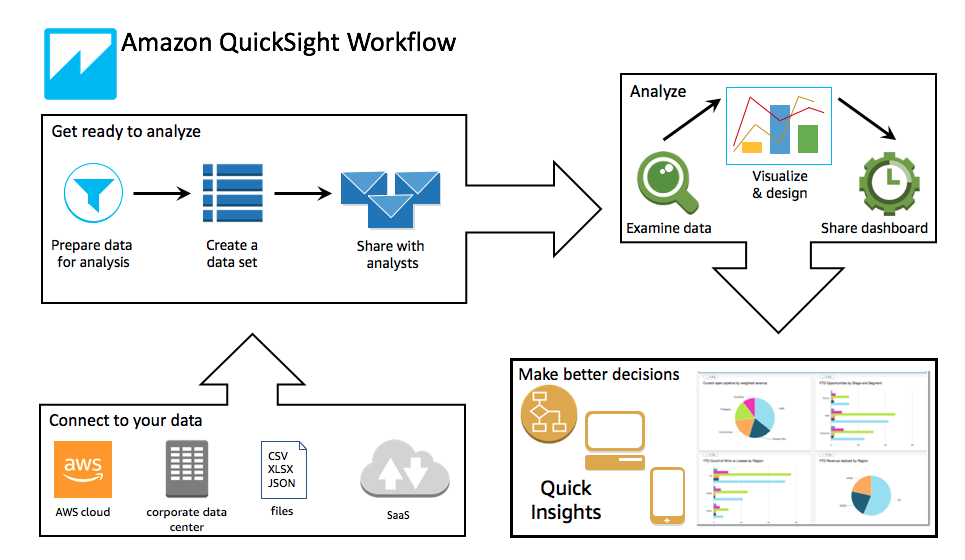
\includegraphics[width=\columnwidth]{images/aws_quicksight}
	\caption{Workflow QuickSight}
	\label{fig:quicksight_workflow}
\end{figure}

Tenemos que preparar la data para su respectivo análisis. Esto podría incluír hacer cambios en: \
\begin{itemize}
	\item Filtrar data que sea más relevante para ti
	\item Renombrar columnas para una mejor lectura
	\item Cambiar algunos tipos de datos por otros
	\item Creando una sql para refinar la data.
\end{itemize}

\subsection{Orígenes de data soportados}
\begin{itemize}
	\item Amazon Athena
	\item Amazon Aurora
	\item Amazon Redshift
	\item Amazon S3
	\item Apache Spark
	\item Google Bigquery
	\item Mysql
\end{itemize}

\subsection{Actualizando la Data}
\begin{description}
	\item[Direct Query:] Si usas esta opción cada vez que tu ingreses al dashboard tu verás que la información está actualizada
	\item[SPICE:] No se actualiza, tienes que de forma manual, eliminar el dataset y volver a crearlo para que pueda tomar la información de nuevo.
\end{description}

\subsection{Precios y Límites}
\begin{description}
	\item[Standard Edition:] Cobro por usuarios y existe una tarifa base, ideal para pequeños equipos o empresas que necesitan crear informes o dashboards básicos
	\item[Enterprise Edition:] Cobro basado en sesiones, una sesión se considera la visita al sitio en un rago de 30 min, tarifa por usuario lector, tienes acceso a mas herramientas de ML, Active Directory
\end{description}

\section{Looker Studio}
\section{Benchmark}

\begin{table}[h!]
\centering
\caption{Comparación entre Power BI, AWS QuickSight y Looker Studio}
\renewcommand{\arraystretch}{1.5} % Aumenta el espacio entre filas
\setlength{\tabcolsep}{5pt} % Aumenta el espacio entre columnas
\begin{tabular}{|l|c|c|c|c|}
\hline
\textbf{Característica} & \textbf{Power BI} & \textbf{AWS QuickSight} & \textbf{Looker Studio} & \textbf{Ganador} \\ \hline
\textbf{Integración con ecosistemas} & Sí & Sí & Sí & Todas \\ \hline
\textbf{Interfaz de usuario} & Sí & Sí & Sí & Looker Studio \\ \hline
\textbf{Manipulación de datos} & Sí & Sí & Sí & Power BI \\ \hline
\textbf{Análisis de datos en tiempo real} & Sí & Sí & Sí & Looker Studio \\ \hline
\textbf{Visualización de datos} & Sí & Sí & Sí & Looker Studio \\ \hline
\textbf{Colaboración} & Sí & Sí & Sí & Power BI \\ \hline
\textbf{Integración de datos} & Sí & Sí & Sí & Power BI \\ \hline
\textbf{Modelado de datos} & Sí & Sí & No & Power BI \\ \hline
\textbf{Precio} & No & Sí & Sí & Looker Studio / AWS QuickSight \\ \hline
\textbf{Comunidad y soporte} & Sí & Sí & No & Power BI \\ \hline
\end{tabular}
\end{table}
    
\section{Conclusión}

Existe una fuerte competencia entre Looker Studio, Power BI, y AWS QuickSight. 
Las tres herramientas destacan en diferentes aspectos de la inteligencia empresarial.

Y podemos decir: 
\begin{itemize}
  \item \textbf{Power BI.} Si el usuario se siente comodo como capacidades avanzadas y se puede justificar el costo ya que Power BI ofrece una manipulación de datos robusta, modelado de datos avanzado, y una comunidad de soporte extensa.
  \item \textbf{Looker Studio.} Ideal para usuarios profundamente integrados en el ecosistema de Google, ofreciendo una interfaz simple y fuertes capacidades de análisis en tiempo real.
  \item \textbf{AWS QuickSight.} Una opción sólida para aquellos en el ecosistema de AWS, proporcionando una fuerte integración y capacidades en tiempo real a un precio competitivo.
\end{itemize}
No hay mejores que otras simplemente la diferencia estará en las capacidades que tiene el usuario de conocer la herramienta y de como enfrenta el problema.


%%
%% The acknowledgments section is defined using the "acks" environment
%% (and NOT an unnumbered section). This ensures the proper
%% identification of the section in the article metadata, and the
%% consistent spelling of the heading.
% \begin{acks}
% To Robert, for the bagels and explaining CMYK and color spaces.
% \end{acks}

%%
%% The next two lines define the bibliography style to be used, and
%% the bibliography file.
\bibliographystyle{ACM-Reference-Format}
\bibliography{bibliography}


%%
%% If your work has an appendix, this is the place to put it.
\appendix

\end{document}
\endinput
%%
%% End of file `sample-sigplan.tex'.